\section{Tutorial -- Optimization}\label{sec.opt.tutorial}

This tutorial is a step-by-step walk through of simulation-based optimization. This tutorial builds on the tutorial in Section \ref{tutorial.sim.flowsheet}.

\begin{enumerate}
	\item Open FOQUS.
	\item Load the FOQUS session from the tutorial ``Creating a Flowsheet with Linked Simulations'' in Section  \ref{tutorial.sim.flowsheet} or if that tutorial has not yet been completed, complete it first.
\end{enumerate}

\subsection{Problem Set Up}
If the simulation runs successfully and the results are reasonable, proceed to define the optimization problem. There are four steps to setting up the optimization problem: (1) select the variables, (2) define samples (optional), (3) define the objective function, and constraints and (4) select and configure the solver.

\begin{enumerate}
	\setcounter{enumi}{2}
	\item Select the \bu{Optimization} button from the toolbar at the top of the Home window (Figure \ref{tut.opt.problem.vars}).  Select the \textbf{\underline{Variables}} tab.
	\item Select ``Decision'' from the drop-down list in the \textbf{\underline{Type}} column as the variable type for all 17 variables shown. If more than 17 variables are shown, the edge connecting the ``BFB'' node to the ``Cost'' node was most likely not configured properly. The scale will automatically change to linear, which is acceptable for most problems.
	\item The \textbf{\underline{Min}}, \textbf{\underline{Max}}, and \textbf{\underline{Value}} columns can be changed. The \textbf{\underline{Min}} and \textbf{\underline{Max}} columns define the lower and upper bounds. The \textbf{\underline{Value}} column specifies the initial point. For this example the defaults are acceptable.
\end{enumerate}

\begin{figure}[H] 
	\begin{center}
		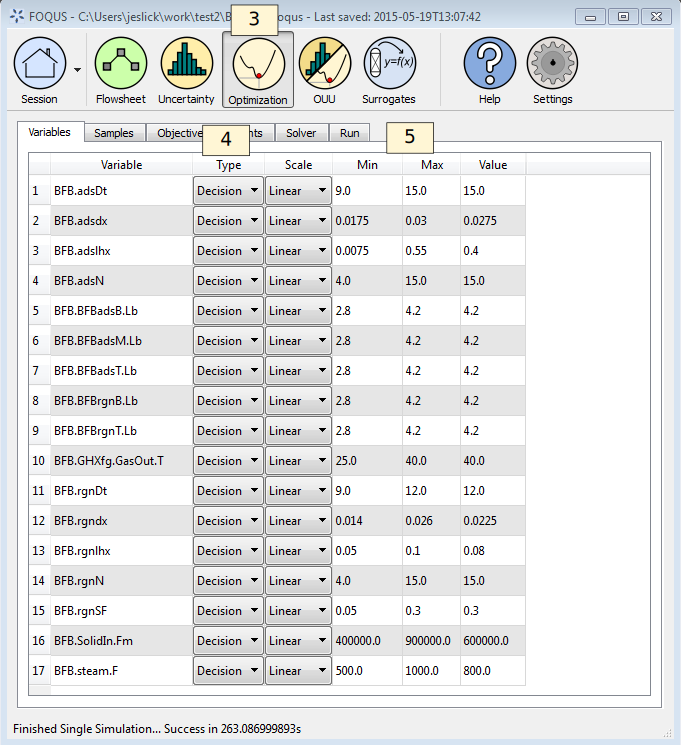
\includegraphics[scale=0.55]{Chapt_optimization/figs/optProblemVar}
		\caption{Optimization Problem Variables}
		\label{tut.opt.problem.vars}
	\end{center}
\end{figure}

If more than one flowsheet evaluation is used in the objective function calculation (e.g., parameter estimation or optimization under uncertainty), the next step is to setup the samples under the \bu{Samples} tab. In this case only one evaluation is used to calculate an objective function value, so the sample setup is not needed. The next step is to define the objective function and constraints using the form under the \textbf{\underline{Objective/Constraints}} tab as shown in Figure \ref{tut.opt.problem.obj}.

\begin{figure}[H] 
	\begin{center}
		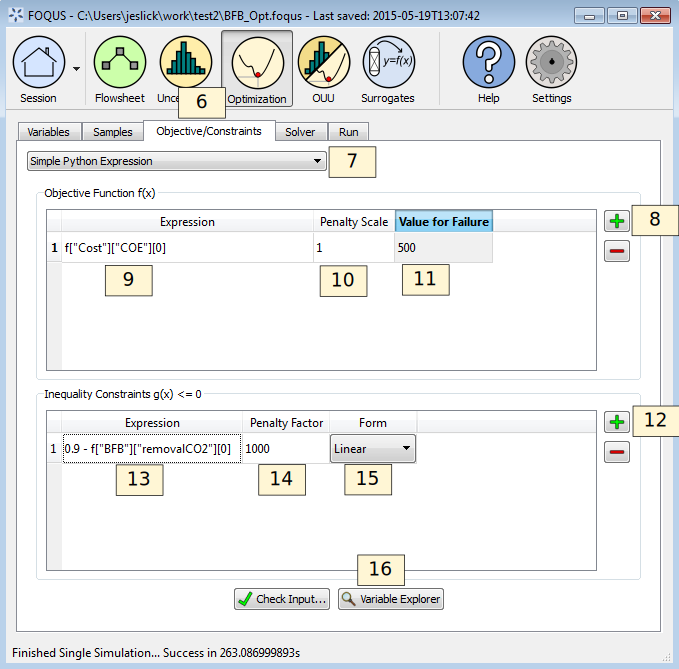
\includegraphics[scale=0.55]{Chapt_optimization/figs/optProblemObj}
		\caption{Optimization Problem Objective}
		\label{tut.opt.problem.obj}
	\end{center}
\end{figure}

\begin{enumerate}
	\setcounter{enumi}{5}
	\item Select the \bu{Objective/Constraints} tab (see Figure \ref{tut.opt.problem.obj}).
	\item In the drop-down list, verify ``Simple Python Expression'' is selected.
	\item Add an objective function by clicking \bu{+} to the right of the Objective Function table.
	\item The objective function is the cost of electricity from the cost spreadsheet.  Enter:\\
	   \verb|f.Cost.COE|\\
	    in the \textbf{\underline{Expression}} column.
	\item Enter 1 in the \textbf{\underline{Penalty Scale}} column. This setting is used mostly for multi-objective optimization to apply the constraint penalty to different objectives.
	\item Enter 500 in the \textbf{\underline{Value for Failure}} column. This should be worse than the objective for any non-failed simulations.
	\item Add a constraint by clicking \bu{+} next to the Inequality Constraints table.
	\item The constraint is that the fraction of CO$_2$ captured must be greater than or equal to 0.9. The constraint is in the form $g(\mathbf{x}) \leq 0$; therefore, in the \textbf{\underline{Expression}} column enter: \\
	 \verb|0.9 - f.BFB.removalCO2|.
	\item Enter 1000 for the \textbf{\underline{Penalty Factor}}.
	\item The constraint penalty \textbf{\underline{Form}} should be linear.
	\item The \textbf{\underline{Variable Explorer}} button can be used to help select flowsheet variables.
\end{enumerate}


\subsection{Solver Settings}
The last step before running the optimization is to select and configure the solver. The solver configuration form is shown in Figure \ref{tut.opt.solver}.

\begin{figure}[H] 
	\begin{center}
		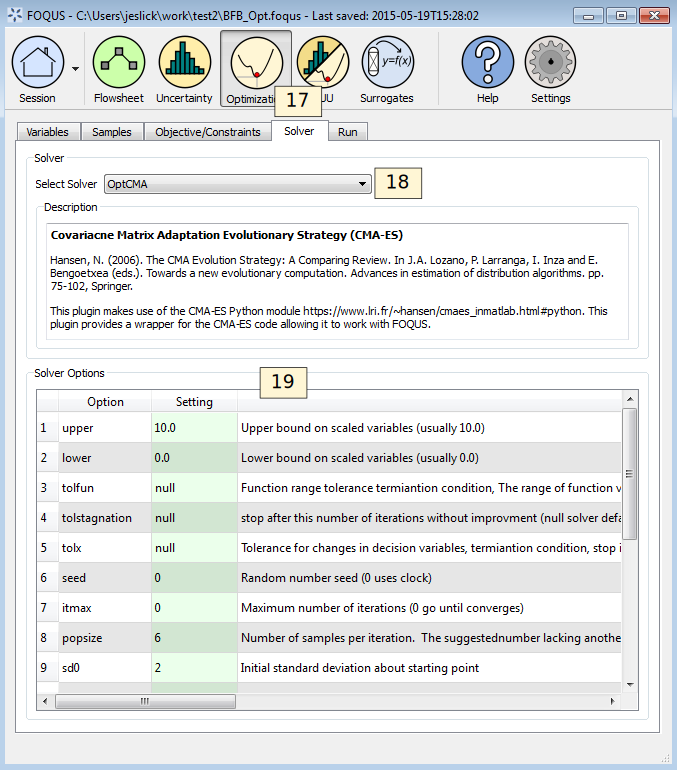
\includegraphics[scale=0.55]{Chapt_optimization/figs/optSolver}
		\caption{Optimization Solver Setup}
		\label{tut.opt.solver}
	\end{center}
\end{figure}

\begin{enumerate}
	\setcounter{enumi}{16}
	\item Select the \bu{Solver} tab (see Figure \ref{tut.opt.solver}).
	\item Select ``OptCMA'' from the \textbf{\underline{Select Solver}} drop-down list.
	\item The default options are acceptable. Solver options are described in the Solver Options table.
\end{enumerate}

\subsection{Running Optimization}

The optimization run form is shown in Figure \ref{tut.opt.run}. 

\begin{figure}[H] 
	\begin{center}
		\includegraphics[scale=0.50]{Chapt_optimization/figs/optRun}
		\caption{Optimization Monitor}
		\label{tut.opt.run}
	\end{center}
\end{figure}

\begin{enumerate}
	\setcounter{enumi}{19}
	\item Click the \bu{Run} tab to display the optimization run form (see Figure \ref{tut.opt.run}).
	\item Click \bu{Start}.
	\item Once the optimization has run for while click \bu{Stop}.
\end{enumerate}

As the optimization run, the best result found is stored in the Flowsheet. If an optimization is run with sample variables the first sample in the set with the best objective function will be stored in the flowsheet. All simulation results can be viewed in the Flowsheet Results table.

The run form displays some diagnostic information as the optimization runs. The parts of the display labeled in Figure \ref{tut.opt.run} are described below.
\begin{enumerate}
	\setcounter{enumi}{22}
	\item The Optimization Solver Messages window displays information from the solver.
	\item The \textbf{\underline{Best Solution Parallel Coordinate Plot}} shows the value of the scaled decision variables, which is useful to see where the best solution is relative to the variable bounds.
	\item The \textbf{\underline{Objective Function Plot}} shows the best value of the objective function found as a function of the optimization iteration or sample number.
	\item While the optimization is running, the status bar shows the amount of time that has elapsed since starting the optimization.
\end{enumerate}
